\chapter{Modelação Conceptual}



\section{Apresentação da abordagem de modelação realizada}

A abordagem escolhida para modelar a base de dados do senhor Miguel baseai-se numa modelação conceptual, que é independente de qualquer implementação que envolva aplicações, linguagens de programação, interfaces de hardware, etc. Para isso, iremos utilizar um modelo abstrato de Entidade-Relacionamento (ER) com a notação de \textbf{Peter Chen} para elaborar um diagrama de entidades, com os seus atributos, e relacionamentos entre elas.\par
Primeiramente, fizemos o levantamento dos elementos principais do nosso modelo, as entidades. Para isso, um dos métodos que usamos foi, por exemplo, analisar os requisitos selecionando os elementos mais destacados.\par
Em segundo lugar, identificamos de que forma as entidades anteriormente selecionadas se relacionam entre si para assim, criar-mos relacionamentos entre elas. Mais uma vez, fizemo-lo  analisando as expressões usadas nos requerimentos levantados.\par
Em terceiro lugar, procedemos à identificação de atributos das entidades ou relacionamentos necessários à base de dados. Para isso identificamos caraterísticas, qualidades e propriedades das varias entidades e relacionamentos, anteriormente levantados, e selecionamos as mais relevantes para o problema em questão.\par
Em quarto lugar, identificamos, para cada atributo, o seu domínio.\par
Em quinto lugar, para cada entidade, selecionamos, entre todos os seus atributos, a melhor chave primária.\par
Seguidamente, verificamos a existência de redundância no nosso modelo, ou seja, analisamos entidade a entidade de forma a confirmar que não tínhamos entidades repetidas, depois focamo-nos nos relacionamentos para garantir que todos eles são imperscindiveis, ou seja, existe pelo menos um caso em que apenas aquele relacionamento me poderia dar acesso àquela informação.\par
Finalmente, procedemos á validação de todo o modelo ao lado do senhor Miguel.

\section{Identificação e caracterização das entidades}
Para identificarmos as várias entidades do nosso modelo conceptual, uma das abordagens tomadas foi a análise rigorosa dos requerimentos levantados. Nomes principais referentes a um ginásio ou objetos os quais sejam bastantes referidos  ou detalhados nos requerimentos feitos pelo senhor Miguel tendem a ser bons candidatos a entidades. \par
Para além disso, procuramos ter em atenção entidades auto suficientes, ou seja, entidades que existem por si próprias, independentes de qualquer outra entidade. Exemplo disso é a entidade Funcionário, pois esta existe, independentemente de sabermos quem são, a sua idade, ou o seu cargo.
Nesta fase, consideramos que a participação e acompanhamento do senhor Miguel foi essencial sendo que, por vezes, foi necessário um melhor esclarecimento dos requisitos de forma a termos um modelo conceptual mais preciso.

\clearpage

\section{Identificação e caracterização dos relacionamentos}

A fim de identificar os vários relacionamentos entre a entidades já anteriormente identificadas iremos mais uma vez  recorrer à  observação dos requerimentos. Desta vez iremos adotar uma análise diferente, que consiste na observação das expressões usadas, focada nos verbos utilizados para relacionar as nossas identidades.\par
Assim, os relacionamentos que selecionamos são:
\vspace{10 pt}


\begin{table}[ht]
\centering
\resizebox{\textwidth}{!}{
\begin{tabular}{|c|c|c|c|}
\hline
Entidade    & Relacionamento      & Entidade    & Cardinalidade \\ \hline
Cliente     & Plano de Exercícios & Exercício   & (0,N) - (0,N) \\ \hline
Cliente     & Tem                 & Fatura      & (1,1) - (0,N) \\ \hline
Cliente     & Subscreve           & Serviço     & (0,N) - (1,N) \\ \hline
Funcionário & Passa               & Fatura      & (1,1) - (1,N) \\ \hline
Equipamento & É utilizado para    & Exercício   & (1,N) - (0,N) \\ \hline
Serviço     & É prestado por      & Funcionário & (0,N) - (0,N) \\ \hline
Serviço     & Constitui           & Fatura      & (1,N) - (0,N) \\ \hline
\end{tabular}
}
\end{table}
\newpage

\section{Identificação e caracterização das Associação dos Atributos
com as Entidades e Relacionamentos.}

No final de reunir todas as entidades e relacionamentos relevantes para o nosso modelo, procedemos então à identificação e caraterização de todos os atributo necessários de modo a cumprir com o requerimentos estabelecidos. Na  tabela 3.1 é possível visualizar todos os atributos de cada entidade e as caraterísticas associadas a cada um deles.

\vspace{10 pt}

\begin{table}[h]
\resizebox{\textwidth}{!}{
\begin{tabular}{|c|ccccccccc|}
\hline
\textbf{Entidade}             & \multicolumn{1}{c|}{\textbf{Atributos}}                        & \multicolumn{1}{c|}{\textbf{Descrição}}                                                                                   & \multicolumn{1}{c|}{\textbf{\begin{tabular}[c]{@{}c@{}}Chave \\ Primária\end{tabular}}} & \multicolumn{1}{c|}{\textbf{Domínio}}                                                                             & \multicolumn{1}{c|}{\textbf{\begin{tabular}[c]{@{}c@{}}Tipo de\\  dados\end{tabular}}} & \multicolumn{1}{c|}{\textbf{Nulo}} & \multicolumn{1}{c|}{\textbf{Multivalor}} & \multicolumn{1}{c|}{\textbf{Composto}} & \textbf{Derivado} \\ \hline
\multirow{17}{*}{Cliente}     & ClienteID                                                      & Identificação do cliente                                                                                                  & Sim                                                                                     & Até 5 dígitos                                                                                                     & INT                                                                                    & Não                                & Não                                      & Não                                    & Não               \\
                              & Nome                                                           & Nome do cliente                                                                                                           & Não                                                                                     & Até 75 caracteres                                                                                                 & VARCHAR(75)                                                                            & Não                                & Não                                      & Não                                    & Não               \\
                              & Idade                                                          & Idade do cliente                                                                                                          & Não                                                                                     & Até 3 dígitos                                                                                                     & INT                                                                                    & Não                                & Não                                      & Não                                    & Não               \\
                              & Morada                                                         & Morada do cliente                                                                                                         & --                                                                                      & --                                                                                                                & --                                                                                     & --                                 & Não                                      & Sim                                    & Não               \\
                              & Localidade                                                     & Localidade do cliente                                                                                                     & Não                                                                                     & Até 75 caracteres                                                                                                 & VARCHAR(75)                                                                            & Não                                & Não                                      & Não                                    & Não               \\
                              & Rua                                                            & Rua do cliente                                                                                                            & Não                                                                                     & Até 75 caracteres                                                                                                 & VARCHAR(75)                                                                            & Não                                & Não                                      & Não                                    & Não               \\
                              & Codigo Postal                                                  & Codigo Postal do Cliente                                                                                                  & Não                                                                                     & \begin{tabular}[c]{@{}c@{}}4 dígitos+\\ 1 caractere "-"+\\ 3 dígitos\end{tabular}                                 & VARCHAR(8)                                                                             & Não                                & Não                                      & Não                                    & Não               \\
                              & Contacto                                                       & Contacto do cliente                                                                                                       & --                                                                                      & --                                                                                                                & --                                                                                     & --                                 & Não                                      & Sim                                    & Não               \\
                              & Telemovel 1                                                     & Nº de telefone do cliente                                                                                                 & Não                                                                                     & 9 dígitos                                                                                                         & INT                                                                                    & Não                                & Não                                      & Não                                    & Não               \\
                              & Telemovel 2                                                     & \begin{tabular}[c]{@{}c@{}}Segundo nº de telefone do \\ cliente\end{tabular}                                              & Não                                                                                     & 9 dígitos                                                                                                         & INT                                                                                    & Sim                                & Não                                      & Não                                    & Não               \\
                              & Email                                                          & Email do cliente                                                                                                          & Não                                                                                     & Até 75 caracteres                                                                                                 & VARCHAR(75)                                                                            & Não                                & Não                                      & Não                                    & Não               \\
                              & IMC                                                            & \begin{tabular}[c]{@{}c@{}}Indice de massa corporal\\  do cliente\end{tabular}                                            & Não                                                                                     & \begin{tabular}[c]{@{}c@{}}Até 4 dígitos\\ (2 decimais)\end{tabular}                                              & DECIMAL(4,2)                                                                           & Não                                & Não                                      & Não                                    & Sim               \\
                              & Peso                                                           & Peso do cliente                                                                                                           & Não                                                                                     & \begin{tabular}[c]{@{}c@{}}Até 5 dígitos\\ (2 decimais)\end{tabular}                                              & DECIMAL(5,2)                                                                           & Não                                & Não                                      & Não                                    & Não               \\
                              & Altura                                                         & Altura do cliente                                                                                                         & Não                                                                                     & \begin{tabular}[c]{@{}c@{}}Até 4 dígitos\\ (2 decimais)\end{tabular}                                              & DECIMAL(4,2)                                                                           & Não                                & Não                                      & Não                                    & Não               \\
                              & Nr Contribuinte                                                & Nº de contribuinte do cliente                                                                                             & Não                                                                                     & 9 dígitos                                                                                                         & INT                                                                                    & Não                                & Não                                      & Não                                    & Não               \\
                              & Sexo                                                           & Sexo do cliente                                                                                                           & Não                                                                                     & 1 caractere (F/M)                                                                                                 & VARCHAR(1)                                                                             & Não                                & Não                                      & Não                                    & Não               \\
                              & Dependencias Fisicas                                           & \begin{tabular}[c]{@{}c@{}}Dependências físicas do \\ cliente\end{tabular}                                                & Não                                                                                     & Até 45 caracteres                                                                                                 & VARCHAR(45)                                                                            & Sim                                & Não                                      & Não                                    & Não               \\ \hline
\multirow{13}{*}{Funcionário} & FuncionárioID                                                  & Identificação do funcionário                                                                                              & Sim                                                                                     & Até 4 dígitos                                                                                                     & INT                                                                                    & Não                                & Não                                      & Não                                    & Não               \\
                              & Nome                                                           & Nome do funcionário                                                                                                       & Não                                                                                     & Até 45 caracteres                                                                                                 & VARCHAR(45)                                                                            & Não                                & Não                                      & Não                                    & Não               \\
                              & Cargo                                                          & \begin{tabular}[c]{@{}c@{}}Cargo que o funcionário \\ ocupa no ginásio\end{tabular}                                       & Não                                                                                     & Até 75 caracteres                                                                                                 & VARCHAR(75)                                                                            & Não                                & Não                                      & Não                                    & Não               \\
                              & Idade                                                          & Idade do funcionário                                                                                                      & Não                                                                                     & Até 3 dígitos                                                                                                     & INT                                                                                    & Não                                & Não                                      & Não                                    & Não               \\
                              & Contacto                                                       & Contacto do funcionário                                                                                                   & --                                                                                      & --                                                                                                                & --                                                                                     & --                                 & --                                       & Sim                                    & Não               \\
                              & Telemovel 1                                                     & Nº do telefone do funcionário                                                                                             & Não                                                                                     & 9 dígitos                                                                                                         & INT                                                                                    & Não                                & Não                                      & Não                                    & Não               \\
                              & Telemovel 2                                                     & \begin{tabular}[c]{@{}c@{}}Segundo nº de telefone do \\ funcionário\end{tabular}                                          & Não                                                                                     & 9 dígitos                                                                                                         & INT                                                                                    & Sim                                & Não                                      & Não                                    & Não               \\
                              & Email                                                          & Email do funcionário                                                                                                      & Não                                                                                     & Até 75 caracteres                                                                                                 & VARCHAR(75)                                                                            & Não                                & Não                                      & Não                                    & Não               \\
                              & Morada                                                         & Morada do funcionário                                                                                                     & Não                                                                                     & --                                                                                                                & --                                                                                     & --                                 & --                                       & Sim                                    & Não               \\
                              & Rua                                                            & Rua onde o funcionário habita                                                                                             & Não                                                                                     & Até 75 caracteres                                                                                                 & VARCHAR(75)                                                                            & Não                                & Não                                      & Não                                    & Não               \\
                              & Localidade                                                     & \begin{tabular}[c]{@{}c@{}}Localidade onde o funcionário \\ habita\end{tabular}                                           & Não                                                                                     & Até 75 caracteres                                                                                                 & VARCHAR(75)                                                                            & Não                                & Não                                      & Não                                    & Não               \\
                              & Codigo Postal                                                  & Código Postal do funcionário                                                                                              & Não                                                                                     & \begin{tabular}[c]{@{}c@{}}4 dígitos+\\ 1 caractere (-)+\\ 3 dígitos\end{tabular}                                 & VARCHAR(8)                                                                             & Não                                & Não                                      & Não                                    & Não               \\
                              & Estado                                                         & \begin{tabular}[c]{@{}c@{}}Estado em que se encontra\\ o funcionário (se ainda\\ trabalha ou não no ginásio)\end{tabular} & Não                                                                                     & 1 caractere (A/N)                                                                                                 & VARCHAR(1)                                                                             & Não                                & Não                                      & Não                                    & Não               \\ \hline
\multirow{4}{*}{Serviço}      & ServçoID                                                       & Identificação do Serviço                                                                                                  & Sim                                                                                     & Até 3 dígitos                                                                                                     & INT                                                                                    & Não                                & Não                                      & Não                                    & Não               \\
                              & Preço                                                          & Preço do Serviço                                                                                                          & Não                                                                                     & \begin{tabular}[c]{@{}c@{}}Até 5 dígitos\\ (2 decimais)\end{tabular}                                              & DECIMAL(5,2)                                                                           & Não                                & Não                                      & Não                                    & Não               \\
                              & Designação                                                     & Especificação do serviço                                                                                                  & Não                                                                                     & Até 45 caracteres                                                                                                 & VARCHAR(45)                                                                            & Não                                & Não                                      & Não                                    & Não               \\
                              & Estado                                                         & \begin{tabular}[c]{@{}c@{}}Estado em que se encontra\\ o funcionário (se ainda\\ trabalha ou não no ginásio)\end{tabular} & Não                                                                                     & 1 caractere (A/N)                                                                                                 & VARCHAR(1)                                                                             & Não                                & Não                                      & Não                                    & Não               \\ \hline
\multirow{6}{*}{Fatura}       & IdFatura                                                       & Identificação da Fatura                                                                                                   & Sim                                                                                     & Até 9 dígitos                                                                                                     & INT                                                                                    & Não                                & Não                                      & Não                                    & Não               \\
                              & \begin{tabular}[c]{@{}c@{}}Contribuinte\\ Ginásio\end{tabular} & \begin{tabular}[c]{@{}c@{}}Nº de contribuinte do\\ Ginásio\end{tabular}                                                   & Não                                                                                     & 9 dígitos                                                                                                         & INT                                                                                    & Não                                & Não                                      & Não                                    & Não               \\
                              & Data                                                           & \begin{tabular}[c]{@{}c@{}}Data de emissão da \\ fatura\end{tabular}                                                      & Não                                                                                     & \begin{tabular}[c]{@{}c@{}}2 dígitos+\\ 1 caractere (/)+\\ 2 dígitos+\\ 1 caractere (/)+\\ 4 dígitos\end{tabular} & DATE                                                                                   & Não                                & Não                                      & Não                                    & Não               \\
                              & Desconto                                                       & \begin{tabular}[c]{@{}c@{}}Desconto associado \\ à fatura\end{tabular}                                                    & Não                                                                                     & \begin{tabular}[c]{@{}c@{}}Até 2 dígitos \\ decimais\end{tabular}                                                 & DOUBLE                                                                                 & Não                                & Não                                      & Não                                    & Não               \\
                              & Descrição                                                      & \begin{tabular}[c]{@{}c@{}}Serviços prestados ao\\ cliente\end{tabular}                                                   & Não                                                                                     & Até 300 caracteres                                                                                                & VARCHAR(300)                                                                           & Não                                & Não                                      & Não                                    & Não               \\
                              & Valor                                                          & \begin{tabular}[c]{@{}c@{}}Valor a ser cobrado\\ pelos serviços prestados\end{tabular}                                    & Não                                                                                     & \begin{tabular}[c]{@{}c@{}}Até 5 dígitos\\ (2 decimais)\end{tabular}                                              & Decimal(5,2)                                                                           & Não                                & Não                                      & Não                                    & Sim               \\ \hline
\multirow{4}{*}{Equipamento}  & idEquipamento                                                  & Identificação de Equipamento                                                                                              & Sim                                                                                     & Até 3 dígitos                                                                                                     & INT                                                                                    & Não                                & Não                                      & Não                                    & Não               \\
                              & Nome                                                           & Nome do equipamento                                                                                                       & Não                                                                                     & Até 45 dígitos                                                                                                    & VARCHAR(45)                                                                            & Não                                & Não                                      & Não                                    & Não               \\
                              & Descrição                                                      & Descrição do equipamento                                                                                                  & Não                                                                                     & Até 75 dígitos                                                                                                    & VARCHAR(75)                                                                            & Não                                & Não                                      & Não                                    & Não               \\
                              & Estado                                                         & \begin{tabular}[c]{@{}c@{}}Estado em que se encontra\\ o funcionário (se ainda\\ trabalha ou não no ginásio)\end{tabular} & Não                                                                                     & 1 caractere (A/N)                                                                                                 & VARCHAR(1)                                                                             & Não                                & Não                                      & Não                                    & Não               \\ \hline
\multirow{3}{*}{Exercício}    & ExercícioID                                                    & Identificação do exercício                                                                                                & Sim                                                                                     & Até 3 dígitos                                                                                                     & INT                                                                                    & Não                                & Não                                      & Não                                    & Não               \\
                              & Designação                                                     & Nome do exercício                                                                                                         & Não                                                                                     & Até 45 dígitos                                                                                                    & VARCHAR(45)                                                                            & Não                                & Não                                      & Não                                    & Não               \\
                              & Tipo de Exercicio                                              & \begin{tabular}[c]{@{}c@{}}Tipo de exercício a ser\\  praticado\end{tabular}                                              & Não                                                                                     & Até 45 dígitos                                                                                                    & VARCHAR(45)                                                                            & Não                                & Não                                      & Não                                    & Não               \\ \hline
\end{tabular}
}
\caption{Identificação e caraterização dos atributos das entidades.}
\end{table}

\newpage

Seguidamente, podemos analisar os atributos dos relacionamentos coletados.

\begin{table}[h]
\resizebox{\textwidth}{!}{
\begin{tabular}{|c|cccccccc|}
\hline
\textbf{Relacionamento}                                                         & \multicolumn{1}{c|}{\textbf{Atributos}}                         & \multicolumn{1}{c|}{\textbf{Descrição}}                                                                        & \multicolumn{1}{c|}{\textbf{Domínio}}                                                                            & \multicolumn{1}{c|}{\textbf{\begin{tabular}[c]{@{}c@{}}Tipo de\\  dados\end{tabular}}} & \multicolumn{1}{c|}{\textbf{Nulo}} & \multicolumn{1}{c|}{\textbf{Multivalor}} & \multicolumn{1}{c|}{\textbf{Composto}} & \textbf{Derivado} \\ \hline
\multirow{2}{*}{\begin{tabular}[c]{@{}c@{}}Plano de \\ Exercícios\end{tabular}} & \begin{tabular}[c]{@{}c@{}}Número de \\ repetições\end{tabular} & \begin{tabular}[c]{@{}c@{}}Número de vezes que o \\ cliente deve repetir determinado\\ exercício\end{tabular}  & 3 dígitos                                                                                                        & INT                                                                                    & Não                                & Não                                      & Não                                    & Não               \\
                                                                                & \begin{tabular}[c]{@{}c@{}}Número de \\ Séries\end{tabular}     & \begin{tabular}[c]{@{}c@{}}Número de vezes que o cliente\\ deve realizar determinada\\ repetição\end{tabular}  & 2 dígitos                                                                                                        & INT                                                                                    & Não                                & Não                                      & Não                                    & Não               \\ \hline
Subscreve                                                                       & \begin{tabular}[c]{@{}c@{}}Data \\ Submissão\end{tabular}       & \begin{tabular}[c]{@{}c@{}}Data em que o cliente \\ subscreve determinado serviço\end{tabular}                 & \begin{tabular}[c]{@{}c@{}}2 dígitos+\\ 1 caractere (/)+\\ 2 dígitos+\\ 1 caractere(/)+\\ 4 dígitos\end{tabular} & DATE                                                                                   & Não                                & Não                                      & Não                                    & Não               \\ \hline
É prestado por                                                                  & Data Início                                                     & \begin{tabular}[c]{@{}c@{}}Data em que o funcionário \\ começou a prestar determinado\\ exercício\end{tabular} & \begin{tabular}[c]{@{}c@{}}2 dígitos+\\ 1 caractere (/)+\\ 2 dígitos+\\ 1 caractere(/)+\\ 4 dígitos\end{tabular} & DATE                                                                                   & Não                                & Não                                      & Não                                    & Não               \\ \hline
\end{tabular}
}
\caption{Identificação e caraterização dos atributos dos relacionamentos.}
\end{table}


Depois de todos os atributos identificados,  já com os seus domínios classificados, procedemos então à seleção da melhor chave primária para cada entidade. Na tabela 3.3 podemos observar todos os atributos de cada entidade os quais consideramos serem candidatos a chave primárias.

\begin{table}[h]
\centering
\begin{tabular}{|c|c|c|}
\hline
Entidade                     & Chave Primária                 & Candidato a chave Primária \\ \hline
\multirow{4}{*}{Cliente}     & \multirow{4}{*}{ClienteID}     & ClienteID                  \\
                             &                                & Telemóvel 1                \\
                             &                                & Email                      \\
                             &                                & Nr Contribuinte            \\ \hline
\multirow{3}{*}{Funcionário} & \multirow{3}{*}{FuncionárioID} & FuncionárioID              \\
                             &                                & Telemóvel 1                   \\
                             &                                & Email                      \\ \hline
\multirow{2}{*}{Serviço}     & \multirow{2}{*}{ServiçoID}     & ServiçoID                  \\
                             &                                & Designação                 \\ \hline
Fatura                       & IdFatura                       & IdFatura                \\ \hline
Equipamento                  & IdEquipamento                  & IdEquipamento              \\ \hline
\multirow{2}{*}{Exercício}   & \multirow{2}{*}{ExercícioID}   & ExercícioID                \\
                             &                                & Designação                 \\ \hline
\end{tabular}
\caption{Identificação de candidatos a chave primária.}
\end{table}

Devido a razões de eficiência, decidimos criar um identificador para cada uma das nossas entidades pois, deste modo conseguimos manipular de forma conveniente o domínio destes, a fim de evitar exageros no número de combinações possíveis referente à chave primária de cada entidade. Exemplo disso é, as entidades cliente, funcionário e fatura possuírem um atributo relacionado a um número de contribuinte o qual é um candidato válido a ser chave primária, no entanto, não se justifica ter uma chave primária com 9 dígitos quando o número de clientes esperado do ginásio não ultrapassa as centenas.


\section{Detalhe ou generalização de entidades}
Para guardar e gerir toda a informação requerida pelo nosso cliente, o senhor Miguel, depois de analisar cuidadosamente os requisitos levantados, selecionamos 6 entidades fundamentais para o bom funcionamento e gestão da nossa base de dados. Estas 6 entidades são caraterizadas como entidades fortes na medida em que, são todas independentes umas das outras e todas elas possuem sentido de existência separadamente.ginásio do senhor Miguel.


\begin{enumerate}
\item \textbf{Cliente}:  A entidade Cliente refere-se aos clientes que estão afiliados ao ginásio do senhor Miguel.
\item \textbf{Funcionário}: Este entidade representa todos os funcionários que realizam qualquer tipo de serviço no ginásio.
\item \textbf{Serviço}: A entidade Serviço, como o nome indica, está relacionada com os vários de serviço disponibilizados pelo ginásio os quais são prestados pelos funcionários aos clientes. Exemplo de serviços são natação, nutrição, Personal Trainer.
\item \textbf{Exercício}: Esta entidade, como é evidente, corresponde aos de exercício que um cliente do ginásio poderá praticar, com ou sem supervisionamento por parte de um funcionário.
\item \textbf{Equipamento}: A entidade equipamento, refere-se aos equipamentos que o ginásio possui os quais podem ser utilizados pelo cliente para praticar exercícios.
\item \textbf{Fatura}: A entidade fatura está relacionada com o pagamento dos serviços prestados no ginásio e como é óbvio, corresponde ás faturas que são impressas pelo ginásio aos clientes do mesmo.
\end{enumerate}


\section{Apresentação e explicação do diagrama ER}
\begin{figure}[h]
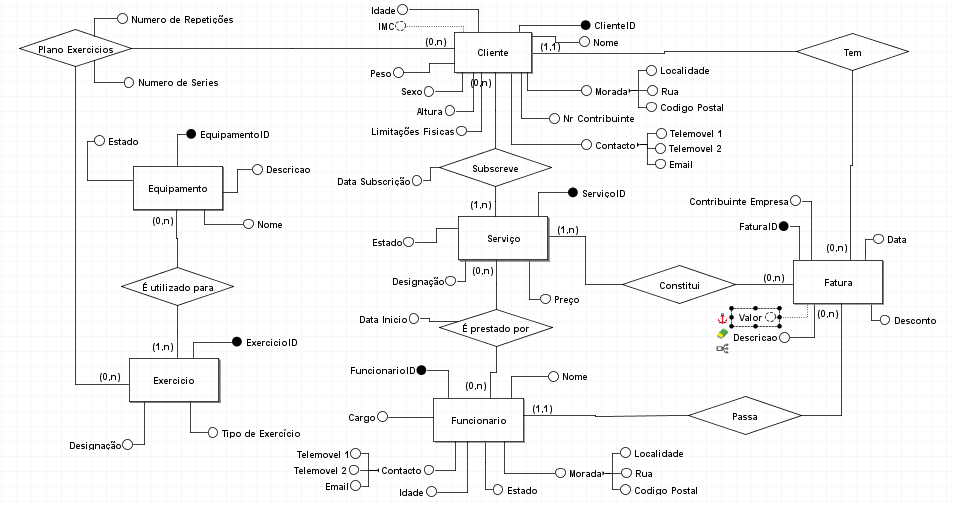
\includegraphics[width=\textwidth]{Conceptual/Conceptual10.png}
\caption{Modelo Conceptual.}
\label{fig:concetual}
\end{figure}

Como já foi dito anteriormente, com o intuito de modelar todas as entidades da nossa base de dados e os relacionamentos entre elas, criamos um diagrama ER usando notação \textbf{Peter Chen} por motivos de organização. Este diagrama é constituído pelas nossas sete entidades as quais estão ligadas entre si através dos relacionamentos já apresentados no grupo 3.3.\par
Uma das razões de se usar um diagrama deste tipo é que este permite-nos chegar a um entendimento mais preciso em relação ao que o senhor Miguel de facto quer / precisa. De facto, é mais fácil visualizar um diagrama de entidades e relacionamentos complexo, do que ler e entender um longo texto com todos os requerimentos do senhor Miguel. Isto acontece pois, por vezes podemos fazer interpretações erradas de alguns requerimentos ou até, o autor dos mesmos pode não os explicar de forma sucinta.\par
Assim, o uso de um diagrama ER permite-nos ter uma visualização do problema bastante mais simplificada e organizada proporcionando-nos uma valiosa ferramenta que será a base de todo este projeto. 

\section{Validação do modelo de dados com o utilizador}

A fim de finalizar todo este processo de modelação, foi necessário que o senhor Miguel o confirmasse e validasse.\par
No final da criação do modelo ER, juntamo-nos mais uma vez com o nosso cliente para, se necessário, retificar alguma gralha no modelo conceptual. 
Alteramos e corrigimos vários detalhes e anomalias referentes ao modelo até que o senhor Miguel ficasse satisfeito.\par
Foi nesta fase que, aquando da aprovação e validação do modelo conceptual como uma  verdadeira representação da realidade na qual o modelo incide (o ginásio), por parte do nosso cliente, este o assinou, marcando assim o fim desta etapa fazendo com que pudéssemos avançar para o modelo lógico.





